\documentclass{beamer}
\usepackage{../common_slides}
\usepackage{tikz-qtree}


\title{Recurrent Neural Networks}
\date{}
\author{CS 287 \\ (Based on Yoav Goldberg's notes)}
\begin{document}


\begin{frame}
  \titlepage
\end{frame}


\begin{frame}{Review: Continuous Bag-of-Bigrams Features?}
  Representation is counts of input bigrams, 
  \begin{itemize}
  \item $\mcF$; the vocabulary of the bigram language.
  \item $\boldx = \sum_{i} \bolddelta(f_i)$ 
  \end{itemize}

  Example: Movie review input, 
  \begin{center}
    \texttt{A sentimental mess}
    \begin{eqnarray*}
      \boldx &=& v(\texttt{word:A})+ v_2(\texttt{bigram:A:sentimental}) \\
      &+&  v(\texttt{word:sentimental}) +   v_2(\texttt{bigram:sentimental:mess})  \\
      &+& v(\texttt{word:mess})
    \end{eqnarray*}

  \end{center}
\end{frame}

\begin{frame}{Review: Convolution Formally}
  

  Let our input be the embeddings of the full sentence, $\boldX \in \reals^{n \times d^0}$ 
  \[\boldX = [v(w_1), v(w_2), v(w_3), \ldots, v(w_n)]\]

  Define a window model as $NN_{window}: \reals^{1\times (\dwin d^0) } \mapsto \reals^{1\times \dhid}$,
  \[NN_{window}(\boldx_{win}) = \boldx_{win} \boldW^1 + \boldb^1   \]

  The convolution is defined as $NN_{conv}: \reals^{n\times d^0} \mapsto \reals^{(n - \dwin + 1) \times \dhid}$, 
  \[NN_{conv}(\boldX) = \tanh \begin{bmatrix}NN_{window}(\boldX_{1:\dwin}) \\   
    NN_{window}(\boldX_{2:\dwin+1}) \\
    \vdots \\ 
    NN_{window}(\boldX_{n-\dwin:n}) \\
  \end{bmatrix}  \]

\end{frame}


\begin{frame}{Review: Pooling}
  \begin{itemize}
  \item Unfortunately $NN_{conv}: \reals^{n\times d^0 } \mapsto
    \reals^{(n - \dwin + 1) \times \dhid}$.
    \air 

  \item Need to map down to $\dout$ for different $n$
    \air 

  \item Recall pooling operations. 
    \air 

  \item Pooling ``over-time'' operations $f: \reals^{n\times m} \mapsto \reals^{1 \times m}  $ 


  \begin{enumerate}
  \item $ f_{max}(\boldX)_{1, j} = \max_{i} X_{i, j} $
  \item $ f_{min}(\boldX)_{1, j} = \min_{i} X_{i, j} $
  \item $ f_{mean}(\boldX)_{1, j} = \sum_i X_{i,j} / n $
  \end{enumerate}

  \end{itemize}

  \[f(\boldX) =  \begin{bmatrix}\Downarrow & \Downarrow  & \ldots \\   
    \Downarrow & \Downarrow & \ldots\\
    & \vdots \\ 
    \Downarrow &\Downarrow & \ldots \\
  \end{bmatrix} = [ \ \ \ldots \ \ ]  \]

  
\end{frame}

\begin{frame}{Review: Convolution Diagram (Kim, 2014)}
  \begin{center}
    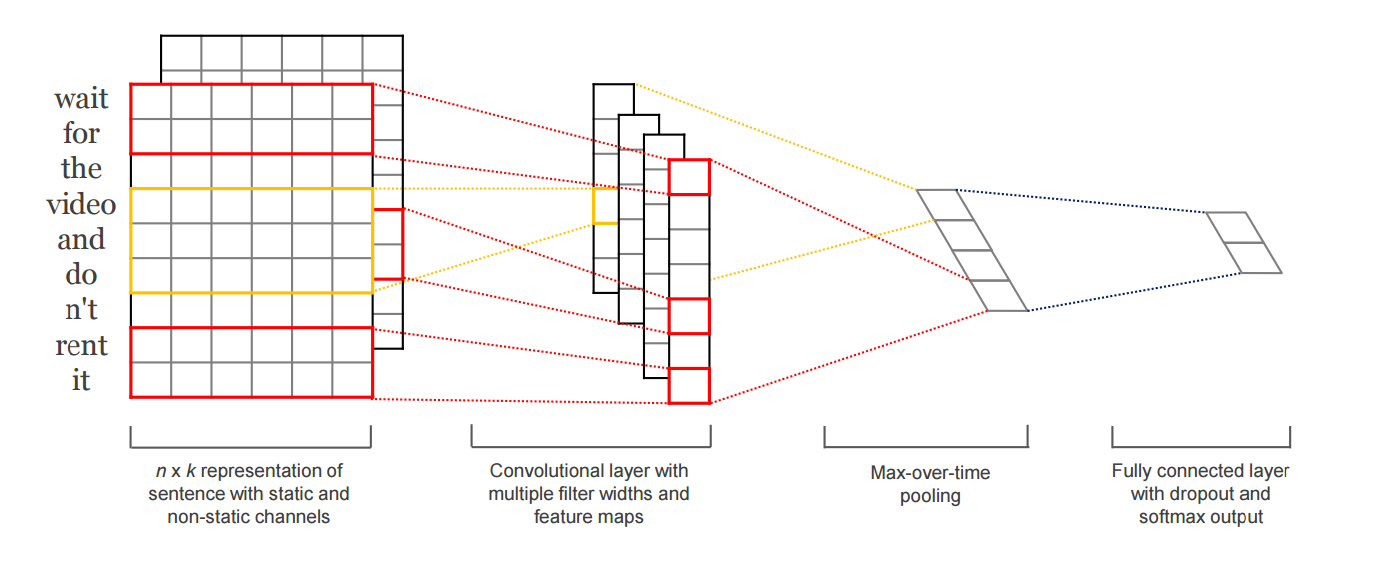
\includegraphics[width=12cm]{kimdiagram}
  \end{center}
  \begin{itemize}
  \item $n = 9$, $\dhid=4$ , $\dout=2$  
    \air 
  \item \alert{red}- $\dwin =2$, \structure{blue}- $\dwin =3$, (ignore back channel) 
    \air 

  \end{itemize}
\end{frame}

\begin{frame}{Quiz}
  Normally when we use a convolution layer we set $\dwin$ to a small
  constant. However you could also set it to degenerate values.
  Describe what model you get when you use the following variants on
  the standard convolution layer. 

  \begin{itemize}

  \item $\dwin=1$ with sparse word features and no pooling or non-linearity. 
    \air 

  \item same as above with sum-over-time pooling
    \air 
  \item $\dwin=n$ (length of sentence) and no pooling. 
  \end{itemize}

\end{frame}

\begin{frame}{Answer}

  \begin{itemize}
  \item This is simply an embedding layer! Here, the number of filters 
    is the same as the embedding size $\demb$.
    \air

  \item This is a continuous bag-of-words model. The convolution 
    acts as the embedding and then the pooling is the sum of the embeddings
    \air 

  \item This is the same as a concatenation of the embedding features followed 
    by a linear layer. The linear layer has different values for each position.
 
  \end{itemize}
  
\end{frame}



\begin{frame}{Representation of Sequence}
  \begin{itemize}
  \item   Many tasks in NLP involve sequences
  \[w_1, \ldots, w_n\] 

  \air
   \item Representations as matrix dense vectors $\boldX$ 

  (Following YG, slight abuse of notation)

  \[\boldx_1 =  \boldx^0_1 \boldW^0, \ldots, \boldx_n =\boldx^0_n \boldW^0 \]

  \item Would like fixed-dimensional representation.
  
  \end{itemize}
\end{frame}

\begin{frame}{Pooling over time?}
  \begin{itemize}
  \item Pooling-over-time gives a fixed-dimensional value.
    \air
  \item However has issues.
    \air
  \item How does convolution help here? What doesn't it do?
  \end{itemize}
\end{frame}

\begin{frame}{Text Classification}

  Consider this (contrived) example:

  \air 
  \texttt{How can you not see this movie?}
  \air 

  \texttt{You should not see this movie.}

  \air
  \begin{itemize}
  \item Would like to classify them differently, despite similar bigrams

    \air

  \item Generally want to have \alert{memory} when making decisions.
  \end{itemize}

\end{frame}

\section{Finite State Machines}

\begin{frame}{Finite State Models}
  \begin{itemize}
  \item Simple, classical way of representing memory

    \air 

  \item Current state representation saves necessary past information.
    \air 
  \end{itemize}
  \textbf{Example:} Email Address Parsing
  \begin{center}
    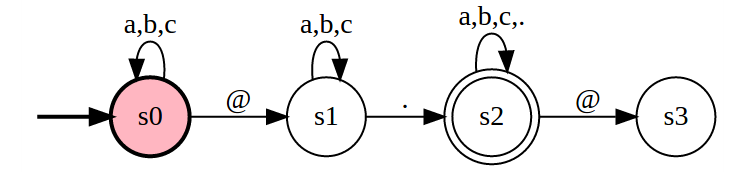
\includegraphics[width=10cm]{email}
  \end{center}

\end{frame}

\begin{frame}{Deterministic Finite State Machine Formally}
  \begin{itemize}
  \item $\mcS$; set of possible states
  \item $\Sigma$; vocabulary
  \item $s_0 \in \mcS$; start state 
  \item $R: (\mcS, \Sigma) \rightarrow \mcS$;  transition function
  \end{itemize}
  \air 
  \begin{itemize}
  \item Maps input $w_1,\ldots,w_n $ to states $s_1, \ldots s_n$ 
  \item For all $i \in \{1,\ldots,n\}$
    \[ s_i = R(s_{i-1}, w_i)\] 
  \end{itemize}
\end{frame}


\begin{frame}{Finite State Machines in NLP}
  \begin{itemize}
  \item words to phonemes in speech
    \air 
  \item n-gram language models
    \air 
  \item manual part-of-speech taggers
    \air
  \item word morphology
  \end{itemize}
\end{frame}

\begin{frame}{Example: Morphology}
  \begin{center}
    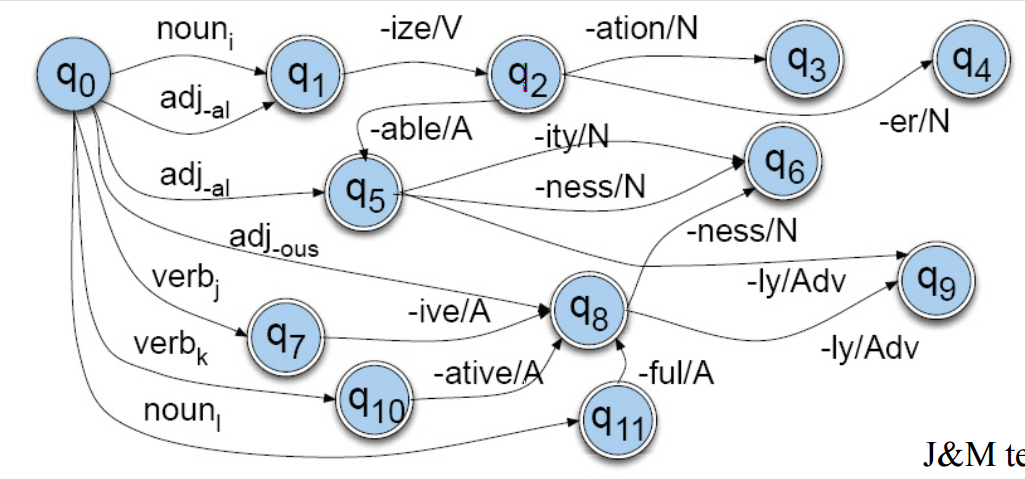
\includegraphics[width=8cm]{morph}
  \end{center}
\end{frame}


\begin{frame}{Variants of State Machines}

  \begin{itemize}
  \item Acceptors; make decision based on final state $s_n$
    \air 

  \item Transducers; apply function $ y_i = O(s_i)$ to produce output at each intermediary state
    \air 

  \item Encoders; utilize last state $s_n$ in another model  
  \end{itemize}
  \air

  Also interesting:
  \begin{itemize}
  \item Ways to learn finite state machine structure
    \air 

  \item Learning weighted finite state machines 
  \end{itemize}
\end{frame}


\section{Recurrent Neural Networks}

\begin{frame}{Recurrent Neural Networks}
  \begin{itemize}
  \item Motivation is to maintain history in the model
    \air

  \item Neural network models with ``memory''
    \air

  \item However no longer finite in the same sense. 
  \end{itemize}
\end{frame}

\begin{frame}{Hidden State}
  \begin{itemize}
    \item  $\mcS = \reals^\dhid$; hidden state space
      \air

    \item  $\Sigma = \reals^\din$ ; input state space
      \air
    \item $s_0 \in \mcS$; initial state vector
      \air

    \item  $R : (\reals^\din \times \reals^\dhid) \mapsto \reals^{\dhid}$; parameterized transition function

  \air       
    \item How might we define $R$?
  \end{itemize}
  \pause

  \[ NN_{elman}(\boldx, \bolds) = \tanh([\boldx, \bolds] \boldW  + \boldb)\]
\end{frame}

% \begin{frame}{Learning the Hidden Representation}

%   \begin{itemize}
%   \item   How do we define $R$? 
%     \air 
    
%   \item 
%   \air 

  
% \item Update is a learned layer of a neural network.
%   \end{itemize}
% \end{frame}

\begin{frame}{Sequence Recurrence}
  \begin{itemize}
  \item Can map from dense sequence to dense representation.

  \item $\boldx_1, \ldots, \boldx_n \mapsto \bolds_1, \ldots, \bolds_n$

  \item For all $i \in \{1, \ldots, n \}$ 

      \[\bolds_{i} = R(\bolds_{i-1}, \boldx_i; \theta) \]
    \item $\theta$ is shared by all $R$
  \end{itemize}

  \textbf{Example:} 
  \begin{eqnarray*}
    \bolds_4 &=& R(\bolds_3, \boldx_4) \\ 
             &=& R(R(\bolds_2, \boldx_3), \boldx_4) \\ 
             &=& R(R(R(R(\bolds_0,\boldx_1), \boldx_2), \boldx_3), \boldx_4) \\ 
  \end{eqnarray*}
\end{frame}


\begin{frame}{RNN versus Convolution and Pooling}
  \begin{columns}
    \column{0.5\textwidth}

    \begin{center}
      \textbf{Convolution}
      \air

      \Tree [ .$Pool$ [ .$NN_{Conv}$ $\boldx_1$ $\boldx_2$ $\ldots$
      $\boldx_n$ ] ]
    \end{center}
    \column{0.5\textwidth}

    \begin{center}
      \textbf{RNN}
      \air 

      \Tree [ .$\bolds_n$ [ .$\ldots$ [ .$\bolds_3$ [ .$\bolds_2$ [ .$\bolds_1$ $\bolds_0$ $\boldx_1$ ]
      $\boldx_2$ ] $\boldx_3$ ] $\ldots$ ] $\boldx_n$ ]
    \end{center}
  \end{columns}
\end{frame}


\begin{frame}{Using Recurrent Neural Networks}
  \begin{itemize}
  \item Hidden states can be applied in different ways.
    \air
  \item Can be used similarly to finite machines
    \begin{itemize}
    \item Acceptor
    \item Transducer
    \item Encoder
    \end{itemize}
  \end{itemize}
\end{frame}

\begin{frame}{Using RNNs: Acceptor}
  \begin{itemize}
  \item Simplest case, sentence acceptor:
    \air 
    \[\hat{boldy} = O(\bolds_n) = \softmax(\bolds_n \boldW + \boldb) \] 

  \item $O: \reals^{\dhid} \mapsto \reals^{\dout}$; final layer

    \air
    
  \item Can be applied to text classification-like tasks
  \end{itemize}

  

\end{frame}


\begin{frame}{Using RNNs: Acceptor Architecture}
  \begin{center}
      \Tree [.$\hat{\boldy}$ [ .$\bolds_n$ [ .$\ldots$ [ .$\bolds_3$ [ .$\bolds_2$ [ .$\bolds_1$ $\bolds_0$ $\boldx_1$ ]
      $\boldx_2$ ] $\boldx_3$ ] $\ldots$ ] $\boldx_n$ ] ]
    \end{center}
\end{frame}

\begin{frame}{Using RNNs: Acceptor (LR version, YG)}
  \begin{center}
    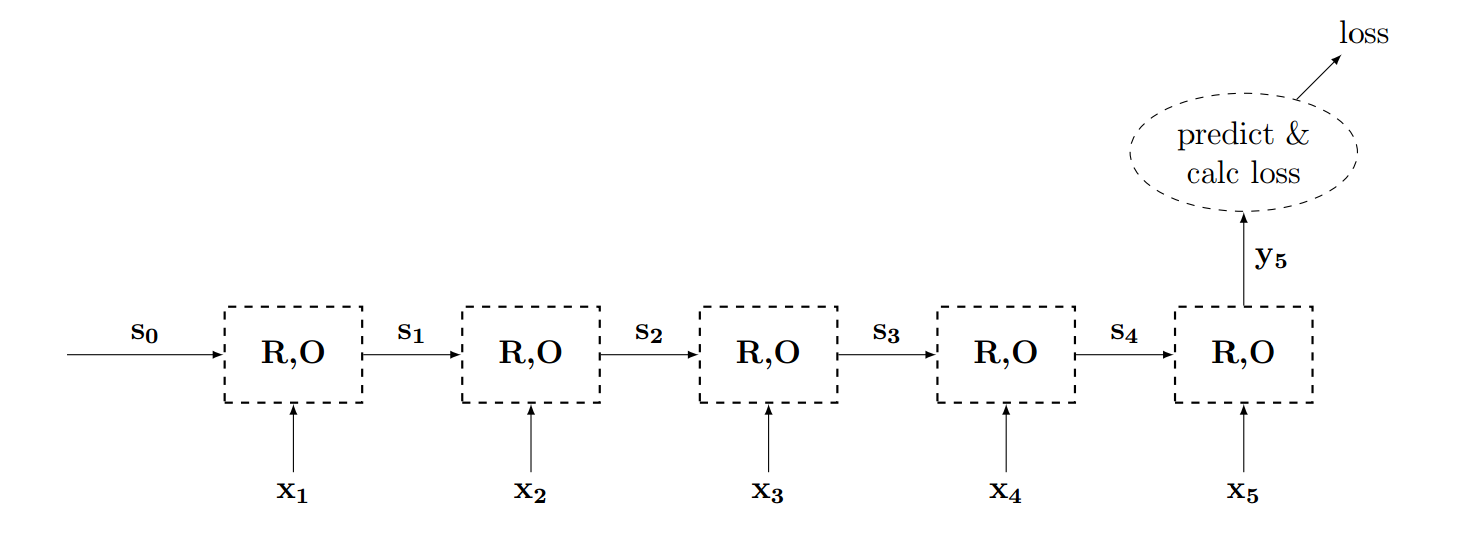
\includegraphics[width=10cm]{ygacceptor}
  \end{center}
\end{frame}

\begin{frame}{Acceptor Versus Convolution}
  \begin{itemize}
  \item In theory, acceptor can model arbitrarily long sequences.
    \air

  \item Memory allows it to incorporate long-range info.
    \air    

  \item Convolution can be run in parallel, multiple dimensions
    \air

  \item Convolution is much shallower, easier to train

  \end{itemize}
\end{frame}

\section{Training RNNs}

\begin{frame}{How do we learn the model?}
  \begin{itemize}
  \item RNNs are trained with SGD and Backprop (surprise)
    \air 

  \item Implementation can be complicated, mainly for efficiency.
    \air

  \item Called \textit{backpropagation through time} (BPTT).
  \end{itemize}
\end{frame}

\begin{frame}{Training Acceptors}
  Training process:
  \begin{itemize}
  \item Run forward propagation.
    \air 
  \item Run backward propagation.
    \air

  \item Update all weights
  \end{itemize}

  Weights $\theta$ of $R$ are shared:

  \[ \frac{\partial L}{\partial \theta} = \sum_{i = 1}^n \frac{\partial L( \ldots R(\boldx_i, \bolds_{i-1})) }{\partial \theta} \] 
\end{frame}

\begin{frame}{BPTT (Acceptor)}
  \begin{itemize}
  \item \alert{Run forward propagation}.
  \item \structure{Run backward propagation}.
  \item Update all weights (shared)
  \end{itemize}

    \begin{center}
      \scalebox{0.7}{\Tree [  .\alert<5->{\structure<6->{$\hat{\boldy}$}} [ .$\alert<4->{\structure<7->{\bolds_n}}$ [ .$\ldots$ [ .$\alert<3->{\structure<8->{\bolds_3}}$ [ .$\alert<2->{\structure<9->{\bolds_2}}$ [ .$\alert<1->{\structure<10->{\bolds_1}}$ $\bolds_0$ $\boldx_1$ ]
      $\boldx_2$ ] $\boldx_3$ ] $\ldots$ ] $\boldx_n$ ] ]}
    \end{center}
\end{frame}

\begin{frame}{Issues}
  \begin{itemize}
  \item Can be inefficient, but batch/GPUs help.
    \air

  \item Model is much deeper than previous approaches.
    \begin{itemize}
    \item This matters a lot, focus of next class.
    \end{itemize}
    \air

  \item Variable-size model for each sentence.
    \begin{itemize}
    \item Have to be a bit more clever in Torch.
    \end{itemize}
  \end{itemize}
\end{frame}

\section{RNN Variants}

\begin{frame}{RNN for Language Modeling}
  \begin{itemize}
  \item Recent popularization of RNNs has been based on language modeling (Mikolov, 2012)
    \air

  \item In particular RNNs allow for non-Markovian models
    \[ p(w_i | w_1, \ldots, w_{i-1};\theta) = O(\bolds_i) \]

    \air 

  \item Compare this to the feed-forward windowed approach.
    \[ p(w_i | w_{i-n+1}, \ldots, w_{i-1};\theta) = O(\bolds_i) \]
  \end{itemize}
\end{frame}


\begin{frame}{RNN as Transducer}
  \begin{center}
  \begin{tikzpicture}
    \node(ya){$\hat{\boldy}_1$}; 

    \node(sa)[below=of ya]{$\bolds_1$}; 
    \node(xa)[below=of sa]{$\boldx_1$}; 
    \node(yb)[right=of ya]{$\hat{\boldy}_2$}; 
    \node(sb)[below=of yb]{$\bolds_2$}; 
    \node(xb)[below=of sb]{$\boldx_2$}; 
    \node(yc)[right=of yb]{$\hat{\boldy}_3$}; 
    \node(sc)[below=of yc]{$\bolds_3$}; 
    \node(xc)[below=of sc]{$\boldx_3$}; 
    \draw (sa) edge (sb); 
    \draw (sb) edge (sc); 


    \draw (sa) -- (xa); 
    \draw (sb) -- (xb); 
    \draw (sc) -- (xc); 
    \draw (sa) -- (ya); 
    \draw (sb) -- (yb); 
    \draw (sc) -- (yc); 
  \end{tikzpicture}
  \end{center}
  \begin{itemize}
  \item Can reuse hidden state each time
    \[ p(w_i | w_1, \ldots, w_{i-1};\theta) = O(\bolds_i) = O(R(\bolds_{i-1}, \boldx_{i})) \]
    \[ p(w_{i+1} | w_1, \ldots, w_{i};\theta) = O(R(\bolds_{i}, \boldx_{i+1})) \]
  \end{itemize}
\end{frame}

\begin{frame}{Transducers Formally}
  \begin{itemize}
  \item Prediction next $\hat{\boldy}_i$ as we go
    \air 
  \item For all $i \in \{1, \ldots, n\}$

    \[\hat{\boldy}_i = O(\bolds_i) = \softmax(\bolds_i \boldW + \boldb) \] 
    \air 
  \item $O: \reals^{\dhid} \mapsto \reals^{\dout}$
  \end{itemize}

\end{frame}

\begin{frame}{BPTT Transducer Training}
  \begin{itemize}
  \item \alert{Run forward propagation}.
  \item \structure{Run backward propagation}
  \item Update all weights (shared)
  \end{itemize}

  \begin{center}
  \begin{tikzpicture}
    \node(ya){$\alert<2->{\structure<7->{\hat{\boldy}_1}}$}; 

    \node(sa)[below=of ya]{$\alert<2->{\structure<7->{\bolds_1}}$}; 
    \node(xa)[below=of sa]{$\boldx_1$}; 
    \node(yb)[right=of ya]{$\alert<3->{\structure<6->{\hat{\boldy}_2}}$}; 
    \node(sb)[below=of yb]{$\alert<3->{\structure<6->{\bolds_2}}$}; 
    \node(xb)[below=of sb]{$\boldx_2$}; 
    \node(yc)[right=of yb]{$\alert<4->{\structure<5->{\hat{\boldy}_3}}$}; 
    \node(sc)[below=of yc]{$\alert<4->{\structure<5->{\bolds_3}}$}; 
    \node(xc)[below=of sc]{$\boldx_3$}; 
    \draw (sa) edge (sb); 
    \draw (sb) edge (sc); 


    \draw (sa) -- (xa); 
    \draw (sb) -- (xb); 
    \draw (sc) -- (xc); 
    \draw (sa) -- (ya); 
    \draw (sb) -- (yb); 
    \draw (sc) -- (yc); 
    \only<2->{\draw (sa) edge[color=red] (ya);  \draw (sa) edge[color=red] (xa); }
    \only<3->{\draw (sa) edge[color=red] (sb);   \draw (sb) edge[color=red] (yb);   \draw (sb) edge[color=red] (xb);}
    \only<4->{\draw (sb) edge[color=red] (sc);  \draw (sc) edge[color=red] (yc); \draw (sc) edge[color=red] (xc);}; 

    \only<7->{\draw (sa) edge[color=blue] (sb); \draw (sa) edge[color=blue] (ya); \draw (sa) edge[color=blue] (xa);}
    \only<6->{\draw (sb) edge[color=blue] (sc); \draw (sb) edge[color=blue] (yb); \draw (sb) edge[color=blue] (xb);} 
    \only<5->{\draw (sc) edge[color=blue] (yc); \draw (sc) edge[color=blue] (xc);}
  \end{tikzpicture}
  \end{center}
\end{frame}

\begin{frame}
  \begin{center}
    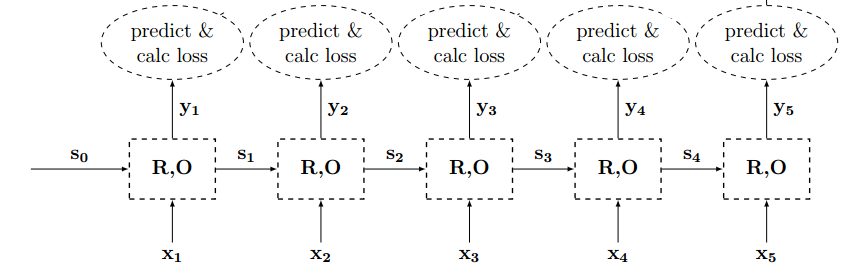
\includegraphics[width=\textwidth]{ygtransducer}
  \end{center}

\end{frame}


\begin{frame}{Bidirectional RNNs}
  \begin{itemize}
  \item RNNs compute a prefix representation.
    \air 

  \item But for tagging we used a bidirectional window. 

    \air 

  \item How can we get a postfix representation?

  \[ w_1 w_2 [\textcolor{red}{w_3 w_4 w_5 w_6 w_7 w_8}] \] 

  \end{itemize}

\end{frame}

\begin{frame}{Bidirectional Models}
  \begin{itemize}
    \item For all $i \in \{1, \ldots, n \}$ 

      \[\bolds^f_{i} = R^{f}(\bolds_{i-1}, \boldx_i) \]

    \item For all $i \in \{1, \ldots, n \}$ 

      \[\bolds^b_{i} = R^{b}(\bolds_{i+1}, \boldx_i) \]

    \item For all $i \in \{1, \ldots, n \}$ 
      \[ \hat{\boldy}_i = O([\bolds^b_{i}, \bolds^f_{i}]) = [\bolds^b_{i}, \bolds^f_{i}] \boldW + \boldb \] 
  \end{itemize}
\end{frame}

\begin{frame}
  \begin{center}
    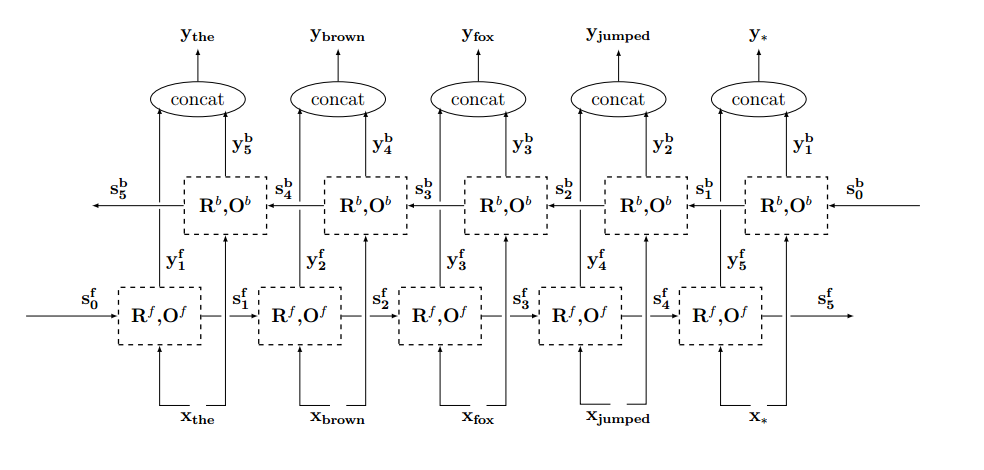
\includegraphics[width=10cm]{ygbidirection}
  \end{center}
\end{frame}


\begin{frame}{Bidirection Models}
  Many applications:
  \begin{itemize}
  \item Tagging
    \air 

  \item Handwriting Recognition (given full sentence)
    \air

  \item Speech Recognition (given full utterance)
    \air 

  \item Machine Translation 
  \end{itemize}
\end{frame}

\end{document}

